\section{ITERAZIONE 1}

In questa prima iterazione di sviluppo viene realizzata la base del sistema: la
struttura architetturale (componenti, interfacce, modello dati e deployment) e le
API REST che coprono il flusso operativo principale  composizione e conferma
degli ordini, gestione del menù, delle scorte e delle stampanti. Le versioni
``intelligenti'' dello smistamento delle stampe (UC5a) e della gestione predittiva
delle scorte (UC5b) vengono affrontate nelle iterazioni successive.

% ============================================================================
\subsection{Casi d'uso implementati}

In questa iterazione vengono implementati i casi d'uso che costituiscono il nucleo
operativo del sistema, descritti nelle \emph{Fully Dressed Descriptions}
dell'Iterazione~0.

\begin{table}[H]
\centering
\caption{Casi d'uso sviluppati nell'Iterazione 1}
\label{tab:uc-iter1}
\begin{tabular}{ll}
\toprule
\textbf{ID} & \textbf{Titolo} \\
\midrule
UC1  & Consultare Allergeni \\
UC2  & Aggiungere Pietanze all'Ordine \\
UC3  & Modificare Pietanza Ordinata \\
UC3b & Aggiungere Note \\
UC4  & Gestione Ordine \\
UC5  & Confermare Ordine \\
UC6  & Configurare Menù \\
UC6a & Impostare Scorte \\
UC6b & Compilare Allergeni \\
\bottomrule
\end{tabular}
\end{table}

\noindent In questa fase lo smistamento delle stampe e l'aggiornamento delle
scorte alla conferma dell'ordine (UC5a e UC5b) sono realizzati nella loro forma
base; l'estensione con i moduli algoritmici dedicati è oggetto delle
Iterazioni~2 e~3.

% ============================================================================
\newpage
\subsection{Diagrammi UML}

%  Component Diagram
\subsubsection{UML Component Diagram}

Il Component Diagram rappresenta i principali componenti del sistema e
le interfacce attraverso cui questi interagiscono. Il sistema è suddiviso
in quattro sottosistemi: \textit{Database}, \textit{Application Logic},
\textit{Client} e \textit{Stampanti}.

Il sottosistema \textit{Application Logic} espone quattro componenti
distinti, ciascuno responsabile di una funzionalità specifica:
\texttt{GestioneOrdini}, \texttt{GestioneMenu}, \texttt{GestioneScorte}
e \texttt{GestioneStampe}. Ogni componente accede al database tramite
la propria interfaccia dedicata (\texttt{OrdiniInterface},
\texttt{MenuInterface}, \texttt{ScorteInterface}, \texttt{StampeInterface})
ed espone a sua volta un'interfaccia verso i livelli superiori.

Il sottosistema \textit{Client} è composto da due componenti:
\texttt{CassaFrontEnd}, che utilizza \texttt{OrdiniMgmt} e
\texttt{MenuLettura}, e \texttt{AdminFrontEnd}, che utilizza
\texttt{MenuMgmt} e \texttt{ScorteMgmt}. L'interfaccia \texttt{MenuLettura}
è separata da \texttt{MenuMgmt} in quanto la cassa necessita
esclusivamente di accesso in lettura al menù, mentre l'amministratore
ha la necessità di modificarne i contenuti.

Il componente \texttt{GestioneStampe} comunica con il sottosistema
\textit{Stampanti} tramite l'interfaccia \texttt{StampeMgmt}, garantendo
il corretto smistamento degli ordini ai reparti di cucina, bar e griglia.

\begin{figure}[H]
  \centering
  
\includegraphics[width=\textwidth]{IT1_component.png}
  \caption{UML Component Diagram}
  \label{fig:component-diagram}
\end{figure}

\newpage

%  Class Diagram per interfacce
\subsubsection{UML Class Diagram Interface}

Il Class Diagram per interfacce dettaglia le operazioni esposte da
ciascuna interfaccia individuata nel Component Diagram. Ogni interfaccia
rappresenta un contratto che i componenti del sistema devono rispettare,
indipendentemente dalla loro implementazione concreta.

\texttt{OrdiniMgmt} espone le operazioni necessarie alla gestione del
ciclo di vita di un ordine: creazione, modifica, eliminazione e
visualizzazione. \texttt{MenuLettura} espone esclusivamente operazioni
di lettura del menù, in linea con il principio del minimo privilegio
applicato alla postazione cassa. \texttt{MenuMgmt} estende le
funzionalità di lettura con operazioni di inserimento, modifica ed
eliminazione delle voci, riservate al pannello di amministrazione.
\texttt{ScorteMgmt} espone le operazioni per la consultazione e
l'aggiornamento delle scorte disponibili. Infine, \texttt{StampeMgmt}
espone le operazioni per l'invio degli ordini alle stampanti di reparto
e per la verifica del loro stato.

\begin{figure}[H]
  \centering
  
\includegraphics[width=0.8\textwidth]{IT1_Class_interface.png}
  \caption{UML Class Diagram per interfacce}
  \label{fig:class-diagram-interfacce}
\end{figure}

\newpage
%  Class Diagram per tipo di dato
\subsubsection{UML Class Diagram per tipo di dato}

Il Class Diagram per tipo di dato rappresenta le entità del dominio
e i relativi attributi su cui si basa la struttura del database.

Le sei classi individuate sono: \texttt{Utente}, che rappresenta
l'operatore del sistema con il proprio ruolo; \texttt{Ordine}, che
modella un ordine associato a un tavolo con il proprio stato e
timestamp; \texttt{Voce}, che rappresenta una singola voce del menù
con nome, prezzo e categoria; \texttt{Scorta}, che tiene traccia
della disponibilità di un prodotto e della sua soglia minima;
\texttt{Stampante}, che identifica una stampante di reparto con il
proprio stato; e \texttt{Allergene}, che descrive un allergene
associabile a una voce del menù.

\begin{figure}[H]
  \centering
  
\includegraphics[width=\textwidth]{IT1_tipo_di_dato.png}
  \caption{UML Class Diagram per tipo di dato}
  \label{fig:class-diagram-tipo-dato}
\end{figure}


%  Deployment Diagram
\newpages
\subsubsection{UML Deployment Diagram}

Il Deployment Diagram mostra la rappresentazione hardware e software
del sistema, evidenziando su quali device vengono eseguiti i componenti
e attraverso quali interfacce questi comunicano tra loro.

Il nodo \textit{MariaDB} ospita il database relazionale ed espone
quattro interfacce verso il Web Server: \texttt{OrdiniInterface},
\texttt{MenuInterface}, \texttt{ScorteInterface} e
\texttt{StampeInterface}. Il nodo \textit{Web Server} contiene i
quattro componenti applicativi \texttt{GestioneOrdini},
\texttt{GestioneMenu}, \texttt{GestioneScorte} e
\texttt{GestioneStampe}, ciascuno marcato come \texttt{«Control»}.
Il nodo \textit{Client} ospita i due componenti \texttt{«Boundary»}
\texttt{CassaFrontEnd} e \texttt{AdminFrontEnd}, raggiungibili tramite
le interfacce \texttt{OrdiniMgmt}, \texttt{MenuLettura},
\texttt{MenuMgmt} e \texttt{ScorteMgmt}. Infine, il nodo
\textit{Stampanti} contiene il componente \texttt{«Boundary»}
\texttt{Stampanti}, collegato al server tramite l'interfaccia
\texttt{StampeMgmt}.

\begin{figure}[H]
  \centering
  
\includegraphics[width=\textwidth]{IT1_deploy.png}
  \caption{UML Deployment Diagram}
  \label{fig:deployment-diagram}
\end{figure}

% ============================================================================

\newpage
\subsection{Test}

\subsubsection{Analisi statica del codice}

A conclusione dell'iterazione, il backend di base è stato sottoposto ad analisi
statica con la regola \texttt{complexity} di \textbf{ESLint} (complessità
ciclomatica) e con \textbf{madge} (accoppiamento tra moduli e dipendenze
circolari). Questa fotografia stabilisce la \emph{baseline} del sistema  prima
dell'introduzione dei moduli algoritmici  rispetto a cui verranno misurati gli
incrementi delle Iterazioni~2 e~3.

\begin{table}[H]
\centering
\caption{Metriche statiche del backend di base (Iterazione~1)}
\label{tab:analisi-base}
\begin{tabular}{lc}
\toprule
\textbf{Metrica} (backend, \texttt{src/}) & \textbf{Valore} \\
\midrule
Complessità ciclomatica massima        & 51 (\texttt{parsaFlusso}) \\
Funzioni con complessità ciclomatica ${}>{}$ 15 & 4 \\
Funzioni totali analizzate             & 67 \\
Moduli accoppiati a \texttt{db.js} ($C_a$) & 7 \\
Dipendenze circolari                   & 0 \\
Righe di codice (SLOC, escluse vuote e commenti) & 1\,506 \\
\bottomrule
\end{tabular}
\end{table}

Il sistema di base è strutturalmente sano: nessuna dipendenza circolare e un
accoppiamento al database contenuto. L'unico punto realmente critico è il parser
del flusso ESC/POS \texttt{parsaFlusso} (complessità 51), seguito dal bootstrap del
server; tutte le altre funzioni restano ampiamente sotto la soglia di 15, come
mostra la Figura~\ref{fig:cc-base}.

\definecolor{baseCol}{HTML}{1F5FA6}
\pgfplotsset{
    basebar/.style={
        xbar, width=\linewidth, bar width=8pt, enlarge y limits=0.25, xmin=0,
        axis x line*=bottom, axis y line*=left, ytick=data,
        nodes near coords, nodes near coords align={horizontal},
        every node near coord/.append style={font=\scriptsize},
        tick label style={font=\small}, xlabel style={font=\small},
    }
}
\begin{figure}[H]
    \centering
    \resizebox{\textwidth}{!}{%
    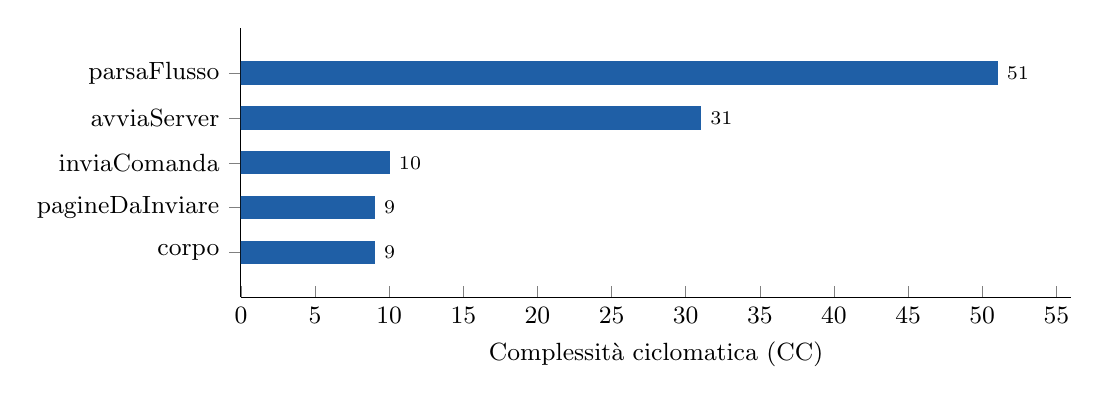
\begin{tikzpicture}
        \begin{axis}[basebar, height=5cm, xmax=56,
            xlabel={Complessità ciclomatica (CC)},
            symbolic y coords={b1,b2,b3,b4,b5},
            yticklabels={corpo, pagineDaInviare, inviaComanda, avviaServer, parsaFlusso},
        ]
            \addplot[fill=baseCol, draw=baseCol] coordinates {(9,b1)(9,b2)(10,b3)(31,b4)(51,b5)};
        \end{axis}
    \end{tikzpicture}%
    }
    \caption{Complessità ciclomatica delle funzioni più impegnative del backend di
    base. Solo \texttt{parsaFlusso} (parser ESC/POS) e il bootstrap del server
    (\texttt{avviaServer}) superano la soglia di 15.}
    \label{fig:cc-base}
\end{figure}

L'accoppiamento tra i moduli e la loro dimensione completano il quadro: i moduli
più connessi sono il bootstrap \texttt{index.js} e la catena di stampa
(Figura~\ref{fig:coupling-base}); i file più estesi restano sotto le 280 righe
(Figura~\ref{fig:sloc-base}).

%  Grafico 2: accoppiamento (fan-out) -
\begin{figure}[H]
    \centering
    \resizebox{\textwidth}{!}{%
    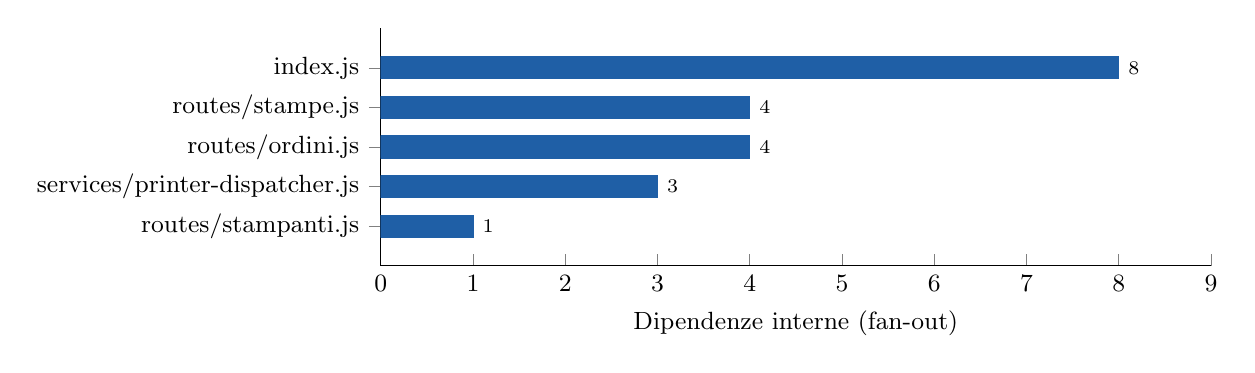
\begin{tikzpicture}
        \begin{axis}[basebar, height=4.6cm, xmax=9,
            xlabel={Dipendenze interne (fan-out)},
            symbolic y coords={k1,k2,k3,k4,k5},
            yticklabels={routes/stampanti.js, services/printer-dispatcher.js,
                         routes/ordini.js, routes/stampe.js, index.js},
        ]
            \addplot[fill=baseCol, draw=baseCol] coordinates {(1,k1)(3,k2)(4,k3)(4,k4)(8,k5)};
        \end{axis}
    \end{tikzpicture}%
    }
    \caption{Accoppiamento: numero di dipendenze interne (fan-out) dei moduli più
    connessi. Complessivamente 7 moduli su 10 dipendono da \texttt{db.js}; nessuna
    dipendenza circolare.}
    \label{fig:coupling-base}
\end{figure}

%  Grafico 3: dimensione dei moduli (SLOC) --
\begin{figure}[H]
    \centering
    \resizebox{\textwidth}{!}{%
    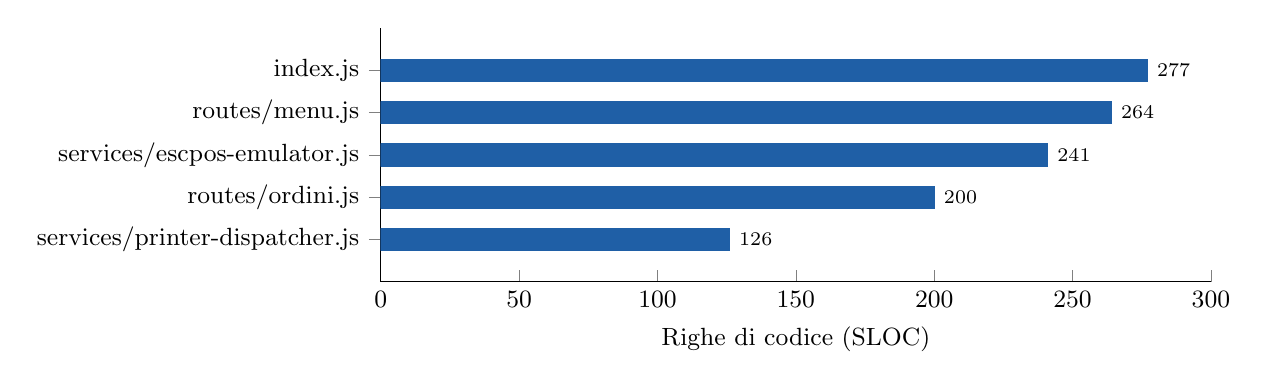
\begin{tikzpicture}
        \begin{axis}[basebar, height=4.8cm, xmax=300,
            xlabel={Righe di codice (SLOC)},
            symbolic y coords={m1,m2,m3,m4,m5},
            yticklabels={services/printer-dispatcher.js, routes/ordini.js,
                         services/escpos-emulator.js, routes/menu.js, index.js},
        ]
            \addplot[fill=baseCol, draw=baseCol] coordinates {(126,m1)(200,m2)(241,m3)(264,m4)(277,m5)};
        \end{axis}
    \end{tikzpicture}%
    }
    \caption{Dimensione dei moduli più grandi del backend di base, in righe di
    codice (SLOC).}
    \label{fig:sloc-base}
\end{figure}

% ============================================================================
\subsubsection{Test automatizzati}

Le funzionalità di base del backend (gestione di ordini, menù, scorte e stampanti)
sono coperte da una suite di test unitari con \textbf{Vitest}, eseguibile con
\texttt{npm test}. La suite conta \textbf{47 test}, tutti superati, distribuiti sui
quattro moduli CRUD; l'esito reale dell'esecuzione è riportato in
Figura~\ref{fig:test-base}.

\begin{figure}[H]
    \centering
    
\includegraphics[width=0.92\textwidth]{IT1_test_base.jpeg}
    \caption{Esecuzione della suite di test del sistema base con Vitest:
             47/47 test superati sui moduli Ordini, Menu, Scorte e Stampanti.}
    \label{fig:test-base}
\end{figure}

I test sono organizzati per risorsa:

\begin{enumerate}
    \item \textbf{Ordini} (12 test). Verificano la creazione, la consultazione e la
    conferma dell'ordine, con calcolo del totale e decremento delle scorte.

    \item \textbf{Menu} (18 test). Coprono la gestione del catalogo: voci visibili e
    nascoste, pietanze aggregate, settori di visualizzazione e associazione degli
    allergeni.

    \item \textbf{Scorte} (10 test). Validano il calcolo dello stato visivo secondo
    le soglie configurate, l'aggiornamento (upsert) della disponibilità e il
    rifornimento.

    \item \textbf{Stampanti} (7 test). Verificano la configurazione delle stampanti
    di reparto: creazione, aggiornamento e rimozione.
\end{enumerate}

% ============================================================================
\subsubsection{API esposte}

Il backend espone quattro risorse principali: \emph{Ordini}, \emph{Menu},
\emph{Scorte} e \emph{Stampanti}. Per tutte valgono le stesse convenzioni, valide
anche per gli endpoint introdotti nelle iterazioni successive: la base URL è
\texttt{http://localhost:3001/api}, lo scambio dati avviene in JSON e gli errori
restituiscono sempre \texttt{\{"errore": "..."\}} con codice HTTP 400, 404, 409 o 500.
Le operazioni di scrittura (\POST, \PUT) sono verificate tramite Postman, di cui
si riporta richiesta e risposta.

% 
\paragraph{Ordini}\mbox{}\\
Gestisce il ciclo di vita degli ordini: creazione, consultazione e conferma con calcolo del totale e aggiornamento delle scorte.

\apicall{\GET~\texttt{/api/ordini}}
Restituisce tutti gli ordini del giorno corrente con righe e note per porzione.

\begin{lstlisting}[style=json]
[
  {
    "id": 1,
    "stato": "confermato",
    "totale": "24.50",
    "importo_pagato": "30.00",
    "timestamp": "2026-04-16T12:30:00.000Z",
    "righe": [
      {
        "voce_id": 3, "quantita": 2, "nome": "Lasagne al forno", "prezzo": "8.50",
        "note": [ { "numero_porzione": 1, "testo": "Senza besciamella" } ]
      }
    ]
  }
]
\end{lstlisting}

\apicall{\GET~\texttt{/api/ordini/:id}}
Dettaglio completo di un singolo ordine. Include \texttt{settore\_stampa} per ogni riga, usato per l'instradamento alla stampante corretta. Risposta \texttt{404} se non trovato.

\begin{lstlisting}[style=json]
{
  "id": 1, "stato": "confermato", "totale": "24.50",
  "righe": [
    {
      "voce_id": 3, "quantita": 2, "nome": "Lasagne al forno",
      "prezzo": "8.50", "settore_stampa": "cucina",
      "note": [ { "numero_porzione": 1, "testo": "Senza besciamella" } ]
    }
  ]
}
\end{lstlisting}

\apicall{\POST~\texttt{/api/ordini}}
Crea un ordine in stato \texttt{in\_composizione}. Richiede almeno una riga con \texttt{voce\_id} e \texttt{quantita}. Va seguito dalla conferma per finalizzarlo.

\postman{i1-ordini-crea.png}{Postman --- \texttt{POST /api/ordini}}

\apicall{\POST~\texttt{/api/ordini/:id/conferma}}
Conferma l'ordine: calcola il totale, decrementa le scorte e porta lo stato a \texttt{confermato}. Emette l'evento WebSocket \texttt{scorte\_aggiornate}.

\postman{i1-ordini-conferma.png}{Postman --- \texttt{POST /api/ordini/:id/conferma}}

% 
\paragraph{Menu}\mbox{}\\
Gestisce il catalogo delle voci, incluse pietanze aggregate (composte da più componenti), settori di visualizzazione e allergeni.

\apicall{\GET~\texttt{/api/menu}}
Voci visibili (\texttt{visibile = 1}) con dati di scorta. Usato dalla cassa per popolare la griglia prodotti.

\begin{lstlisting}[style=json]
[
  {
    "id": 1, "codice": "P001", "nome": "Risotto ai funghi", "prezzo": "9.00",
    "categoria": "Primo", "settore_visualizzazione": "Primi",
    "settore_stampa": "cucina", "colore_tasto": "#E8A838",
    "visibile": 1, "asportabile": 1,
    "scorta_quantita": 45, "soglia_giallo": 10, "soglia_rosso": 3, "scorta_attiva": 1
  }
]
\end{lstlisting}

\apicall{\GET~\texttt{/api/menu/tutte}}
Come \texttt{/api/menu} ma include le voci nascoste e il campo \texttt{num\_componenti} per identificare le pietanze aggregate. Usato dal pannello Admin.

\apicall{\POST~\texttt{/api/menu}}
Crea una nuova voce. Il codice è auto-generato (\texttt{<iniziale-categoria><progressivo>}, es.\ \texttt{P007}). Campo obbligatorio: \texttt{nome}.

\postman{i1-menu-crea.png}{Postman --- \texttt{POST /api/menu}}

\apicall{\PUT~\texttt{/api/menu/:id}}
Aggiornamento parziale: si inviano solo i campi da modificare. Modificabili: \texttt{nome}, \texttt{prezzo}, \texttt{categoria}, \texttt{settore\_visualizzazione}, \texttt{settore\_stampa}, \texttt{colore\_tasto}, \texttt{ordine\_schermo}, \texttt{visibile}, \texttt{asportabile}, \texttt{modalita\_stampa}.

\postman{i1-menu-modifica.png}{Postman --- \texttt{PUT /api/menu/:id}}

\apicall{\DELETE~\texttt{/api/menu/:id}}
Elimina una singola voce. Operazione irreversibile.

% 
\paragraph{Scorte}\mbox{}\\
Gestisce la disponibilità in tempo reale, con stato visivo calcolato automaticamente secondo le soglie configurate per voce.

\vspace{0.3em}
\begin{tabular}{ll}
\toprule
\textbf{Condizione} & \textbf{stato\_visivo} \\
\midrule
\texttt{quantita = 0} & \texttt{esaurito} \\
\texttt{quantita <= soglia\_rosso} (default 3) & \texttt{critico} \\
\texttt{quantita <= soglia\_giallo} (default 10) & \texttt{attenzione} \\
altrimenti & \texttt{disponibile} \\
\bottomrule
\end{tabular}
\vspace{0.5em}

\apicall{\GET~\texttt{/api/scorte}}
Tutte le scorte attive con stato visivo calcolato.

\begin{lstlisting}[style=json]
[
  {
    "voce_id": 1, "nome": "Risotto ai funghi", "codice": "P001",
    "quantita": 8, "soglia_giallo": 10, "soglia_rosso": 3,
    "attiva": 1, "stato_visivo": "attenzione"
  }
]
\end{lstlisting}

\apicall{\GET~\texttt{/api/scorte/:voce\_id}}
Scorta di una singola voce. Ritorna \texttt{null} se non configurata.

\apicall{\PUT~\texttt{/api/scorte/:voce\_id}}
Imposta o sovrascrive (upsert) la scorta. Richiede \texttt{quantita}. Emette \texttt{scorte\_aggiornate} via WebSocket.

\postman{i1-scorte-set.png}{Postman --- \texttt{PUT /api/scorte/:voce\_id}}

\apicall{\POST~\texttt{/api/scorte/:voce\_id/rifornimento}}
Aggiunge unità alla scorta e registra l'operazione nello storico. La \texttt{quantita} deve essere maggiore di zero. Emette \texttt{scorte\_aggiornate} via WebSocket.

\postman{i1-scorte-rifornimento.png}{Postman --- \texttt{POST /api/scorte/:voce\_id/rifornimento}}

% 
\paragraph{Stampanti}\mbox{}\\
Gestisce le stampanti ESC/POS in rete locale, raggruppate per reparto (\texttt{cucina}, \texttt{bar}, \texttt{griglia}).

\apicall{\GET~\texttt{/api/stampanti}}
Lista di tutte le stampanti configurate.

\begin{lstlisting}[style=json]
[
  { "id": 1, "reparto": "cucina", "indirizzo_ip": "192.168.1.101", "porta": 9100, "stato": "sconosciuto" }
]
\end{lstlisting}

\apicall{\POST~\texttt{/api/stampanti}}
Aggiunge una nuova stampante. Obbligatori: \texttt{reparto} e \texttt{indirizzo\_ip}. Porta default: \texttt{9100}.

\postman{i1-stampanti-crea.png}{Postman --- \texttt{POST /api/stampanti}}

\apicall{\PUT~\texttt{/api/stampanti/:id}}
Aggiorna i dati di una stampante. Body identico al POST.

\postman{i1-stampanti-modifica.png}{Postman --- \texttt{PUT /api/stampanti/:id}}

\apicall{\DELETE~\texttt{/api/stampanti/:id}}
Rimuove una stampante dalla configurazione.

\newpage